\vspace{1cm}
\fancyhead[C]{\normalsize\textbf{$\qquad$ Teil I: Offene Aufgaben}}
\renewcommand{\labelenumi}{\theenumi.}
\section*{Aufgabe 1 (38 Punkte)}
\vspace{0.4cm}
%\titleformat{\subsection}[runin]
%{\normalfont\large\bfseries}{\thesubsection}{1em}{}
\subsection*{\aufgabe{a1}{8}} 
Die durchschnittlichen jährlichen Stromkosten eines Schweizer Haushalts sind von ungefähr $800$ Schweizer Franken im Jahr $2012$ auf (voraussichtlich) $1'200$ Schweizer Franken im Jahr $2023$ gestiegen. Um diese Entwicklung darzustellen, nehmen wir an, dass sich die Kosten $C$ über die Zeit gemäss dem folgenden mathematischen Modell entwickeln:
\begin{align*}
	C_\lambda(t)
	=
	\frac{1600}{1 + e^{-\lambda t}},
\end{align*}
wobei $t \geq 0$ die Anzahl der Jahre \textit{nach} $2012$ entspricht und $\lambda = 0.1$.
\\
\\
Nehmen wir an, dass man die Preisentwicklung durch eine Verbesserung der Energieeffizienz entgegenwirken kann, was durch den Parameter $\lambda$ ausgedrückt wird. Das heisst, die Kosten im Jahr $2023$ können beschrieben werden als:
\begin{align*}
	c_{2023}(\lambda) 
	=
	\frac{1600}{1 + e^{- \lambda (2023 - 2012)}}.
\end{align*}
Zeigen Sie, dass es genau einen Wert $\lambda^\star \in [0,0.1]$ gibt, bei dem die Kosten im Jahr $2023$ $1'000$ Schweizer Franken entsprechen.
\
\\ \\
\textbf{Lösung:}
\begin{mdframed}
\underline{\textbf{Vorgehensweise:}}
\renewcommand{\labelenumi}{\theenumi.}
\begin{enumerate}
\item 
Stelle den mathematischen Rahmen her.
\item
Überlege wie man die Existenz und Eindeutigkeit zeigt.
\item
Wende den Nullstellensatz von Bolzano an und zeige die Eindeutigkeit. 
\end{enumerate}
\end{mdframed}
\underline{1. Stelle den mathematischen Rahmen her}\\
Zunächst werden wir den mathematischen Rahmen herstellen. Damit wissen wir welches Problem angegangen wird und wir können die passenden Konzepte anwenden.\\
\\
Diese Aufgabe sucht nach der Existenz und Eindeutigkeit eines Wertes $\lambda^\star \in [0,0.1]$, für welchen die jährlichen Stromkosten eines Schweizer Haushalts im Jahr 2023 $1000$ Schweizer Franken betragen.
Nach der Aufgabe sind diese Kosten durch $c_{2023}(\lambda)$ in Abhängigkeit von $\lambda$ gegeben (Effizienzparameter).
Gesucht ist also der eindeutige Wert $\lambda^\star \in [0,0.1]$, sodass 
\begin{align*}
	c_{2023}(\lambda) = 1000
	\ \Leftrightarrow \ 
	c_{2023}(\lambda) - 1000 = 0
\end{align*}
gilt. Damit erhalten wir mit 
\begin{align*}
	f(\lambda) := c_{2023}(\lambda) - 1000 
	=
	\frac{1600}{1 + e^{- \lambda (2023 - 2012)}} - 1000
	=
	\frac{1600}{1 + e^{- \lambda\cdot 11}} - 1000
\end{align*}
das Nullstellenstellenproblem
\begin{align*}
	f(\lambda^\star) = 0.
\end{align*}
Zu zeigen ist also, dass eine eindeutige Lösung $\lambda^\star$ in dem Intervall $[0, 0.1]$ existiert.\\
\\
\underline{2. Überlege wie man die Existenz und Eindeutigkeit zeigt}\\
Um zu zeigen, dass ein $\lambda^\star  \in [0,0.1]$ mit
\begin{align*}
	c_{2023}(\lambda^\star) = 0
\end{align*}
existiert. Hierfür können wir den Nullstellensatz von Bolzano anwenden. Dieser besagt:\\
Sei $f:[a,b] -> \R$ eine stetige Funktion mit $f(a) < 0 \wedge f(b) > 0 $ oder $f(a) > 0 \wedge f(b) < 0$\\
Dann existiert mindestens ein $\lambda^\star \in [a,b]$, sodass $f(\lambda^\star) = 0$ gilt.\\
\\
Damit wissen wir jedoch nur, dass eine Nullstelle existiert. Es könnten auch mehrere Nullstellen in $[0,0.1]$ existieren. 
Falls $f $ auf $[0,0.1]$ streng monoton ist, kann es jeder Wert auf diesem Intervall nur einmal getroffen werden und wir erreichen die Eindeutigkeit.\\
\\
\underline{3. Wende den Nullstellensatz von Bolzano an und zeige die Eindeutigkeit}\\
Die Funktion $f$ ist als Zusammensetzung stetiger Funktionen stetig. Des weiteren gilt:
\begin{align*}
	f(0) = c_{2023}(0) -1000 
	=
	\frac{1600}{1 + e^{-0 \cdot 11} } - 1000
	= 
	\frac{1600}{2} - 1000
	= 
	800 - 1000 = -200 < 0\\
	f(0.01) = c_{2023}(0.1) -1000 
	=
	\frac{1600}{1 + e^{-0.1 \cdot 11} } - 1000
	\approx
	= 
	200.416 > 0.
\end{align*}
Damit existiert mindestens ein $\lambda^\star \in [0,0.1]$, sodass $f(\lambda^\star) = 0$ gilt.\\ 
Für die strenge Monotonie betrachten wir die Ableitung von $f$. Mit der Kettenregel erhalten wir:
\begin{align*}
	f^\prime(\lambda)
	&=
	1600 \cdot (-11) \cdot e^{-11\cdot \lambda } \frac{-1}{\left(1 + e^{-11 \lambda}\right)^2}
	=
	\frac{1600 \cdot 11}{e^{11 \cdot \lambda} \left(1 + e^{-11 \lambda}\right)^2}
	=
	\frac{17600}{e^{\frac{11 \cdot \lambda}{2} \cdot 2} \left(1 + e^{-11 \lambda}\right)^2}\\
	&=
	\frac{17600}{\left(e^{\frac{11 \cdot \lambda}{2}  }\right)^2 \left(1 + e^{-11 \lambda}\right)^2}
	=
	\frac{17600}{\left(\left(e^{\frac{11 \cdot \lambda}{2}  }\right) \left(1 + e^{-11 \lambda}\right) \right)^2}
	=
	\frac{17600}{\left( e^{\frac{11 \cdot \lambda}{2}} + e^{\frac{-11 \cdot \lambda}{2}} \right)^2}.
\end{align*}
Wegen der Positivität der Exponentialfunktion gilt $f^\prime (\lambda) > 0 $ für alle $\lambda \in \R$. Insbesondere gilt dies für unser Intervall $[0,0.1]$.\\
\\
Insgesamt existiert eine eindeutige Lösung $\lambda^\star \in [0,0.1]$, sodass 
\begin{align*}
	f(\lambda^\star) = 0
	\ \Leftrightarrow \
	c_{2023}(\lambda^\star)  = 1000
\end{align*}
gilt. Die Gleichung $c_{2023}(\lambda^\star)$ lässt sich durch
\begin{align*}
	c_{2023}(\lambda^\star)  = 1000
	&\ \Leftrightarrow \
	\frac{1600}{1 + e^{- \lambda^\star \cdot 11}} = 1000
	\ \Leftrightarrow \
	1600 = 1000 + 1000 e^{- \lambda^\star \cdot 11}\\
	&\	\Leftrightarrow \
	1000 e^{- \lambda^\star \cdot 11} = 600\\
	&\	\Leftrightarrow \
	e^{- \lambda^\star \cdot 11} = \frac{6}{10} = \frac{3}{5}
	\ \Leftrightarrow \
	- \lambda^\star \cdot 11 = \ln \left(\frac{3}{5}\right)\\
	&\ \Leftrightarrow \
	\lambda^\star = \frac{\ln(3) - \ln(5)}{-11} \approx 0.04644.
\end{align*}
auch explizit auflösen.

\newpage

\subsection*{\aufgabe{a2}{8}}
Die durchschnittlichen jährlichen Stromkosten eines Schweizer Haushalts sind von ungefähr $800$ Schweizer Franken im Jahr $2012$ auf (voraussichtlich) $1'200$ Schweizer Franken im Jahr $2023$ gestiegen. Um diese Entwicklung darzustellen, nehmen wir an, dass sich die Kosten $C$ über die Zeit gemäss dem folgenden mathematischen Modell entwickeln:
\begin{align*}
	C_\lambda(t)
	=
	\frac{1600}{1 + e^{-\lambda t}},
\end{align*}
wobei $t \geq 0$ die Anzahl der Jahre \textit{nach} $2012$ entspricht und $\lambda = 0.1$.
\\
\\
Nehmen wir an, dass man die Preisentwicklung durch eine Verbesserung der Energieeffizienz entgegenwirken kann, was durch den Parameter $\lambda$ ausgedrückt wird. Das heisst, die Kosten im Jahr $2023$ können beschrieben werden als:
\begin{align*}
	c_{2023}(\lambda) 
	=
	\frac{1600}{1 + e^{- \lambda (2023 - 2012)}}.
\end{align*}
Verwenden Sie eine Taylor-Approximation zweiter Ordnung im Punkt $ \lambda_0 = 0.5 $, um eine Näherung für $ \lambda^\star $ zu finden.
\\
 \\
\textbf{Lösung:}
\begin{mdframed}
\underline{\textbf{Vorgehensweise:}}
\renewcommand{\labelenumi}{\theenumi.}
\begin{enumerate}
\item Bestimme das Taylorpolynom. 
\end{enumerate}
\end{mdframed}

\underline{1. Bestimme das Taylorpolynom}\\

\newpage
\subsection*{\aufgabe{b}{12}}
Sam begeistert sich für non-fungible tokens (NFTs).
Er beschliesst ein digitales Kunstwerk zu kaufen, da er fest daran glaubt, dass der Wert des Kunstwerks innerhalb der nächsten Jahre signifikant steigen wird. 
Das NFT Kunstwerk kostet $100'000$ Schweizer Franken und Sam
beschliesst, sich einen Teil des Geldes für die Finanzierung zu leihen.
Eine Freundin, Caroline, willigt ein, ihm zum 1. Januar 2023 $60'000$
Schweizer Franken zu leihen, wodurch $60 \% $ der Kosten gedeckt werden.
Allerdings verlangt sie einen recht hohen jährlichen Zinssatz
von $5 \%$, da sie Sams Investitionsvorhaben eher skeptisch gegenübersteht.
Darüber hinaus besteht sie darauf, dass Sams Schulden bis Ende des Jahres 2025 auf
$30'000$ Schweizer Franken gesunken und schliesslich bis Ende des Jahres 2028 vollständig getilgt sind.
Um diese Bedingungen zu erfüllen, stimmt Sam zu, dass er jedes Jahr, jeweils am Jahresende, bis zum 31. Dezember 2025 $C_1$ zurückzahlt und $C_2 = 5'000$ Schweizer Franken am Ende jeden Jahres vom 1. Januar 2026 bis zum 31. Dezember 2028.
Die verbleibenden Schulden am Ende des Jahres 2028 will er dann mit dem durch den Verkauf des Kunstwerks generierten
Erlös zurückzahlen.
\begin{enumerate}
	\item[(b1)] Fügen Sie die Ereignisse und Mittelflüsse dem Zeitstrahl hinzu.
	\item[(b2)] Bestimmen Sie die jährlichen Zahlungen $C_1$ jeweils am Ende der Jahre 2023, 2024 und 2025.
	\item[(b3)] Bestimmen Sie die Restschuld am Ende des Jahres 2028 \textit{bevor} Sam das Kunstwerk verkaufen und die Schulden vollständig tilgen wird.
	\item[(b4)] Angenommen Sams Erwartungen bezüglich der Wertentwicklung seines NFT Kunstwerks waren falsch und das Kunstwerk hat seit 1. Januar 2023 jährlich $3 \%$ an Wert verloren. Prüfen Sie, ob es Sam möglich ist, seine Schulden vollständig zurückzuzahlen, wenn er \textit{ausschliesslich} seine Einnahmen aus dem Verkauf des Kunstwerks dafür verwendet.
\end{enumerate}
\begin{center}
	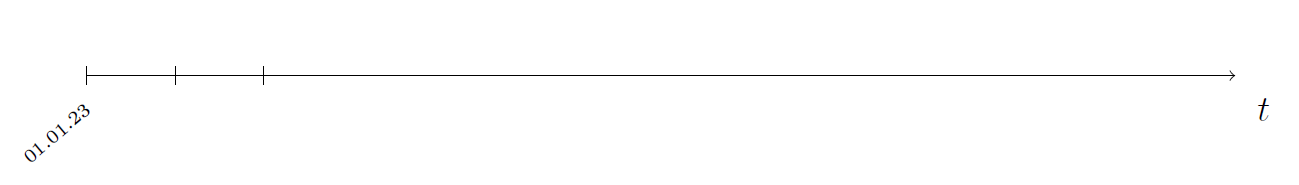
\includegraphics[scale=0.45]{pictures/zeitstrahl_1_b}
\end{center}
\ \\
\textbf{Lösung:}
\begin{mdframed}
\underline{\textbf{Vorgehensweise:}}
\begin{enumerate}
\item[(b1)] Füge den Kredit und die Raten zum Zeitstrahl hinzu.
\item[(b2)] Bestimme die Höhe der Ratenzahlung $ C $.
\item[(b3)] Ergänze den Lottogewinn und berechne die Restschuld.
\item[(b4)] Bestimme die restliche Laufzeit mit Hilfe der Restschuld.
\item[(b5)] Bestimme die letzte Rate.
\end{enumerate}
\end{mdframed}

\newpage
\underline{(b1) Füge den Kredit und die Raten zum Zeitstrahl hinzu}\\
\begin{center}
	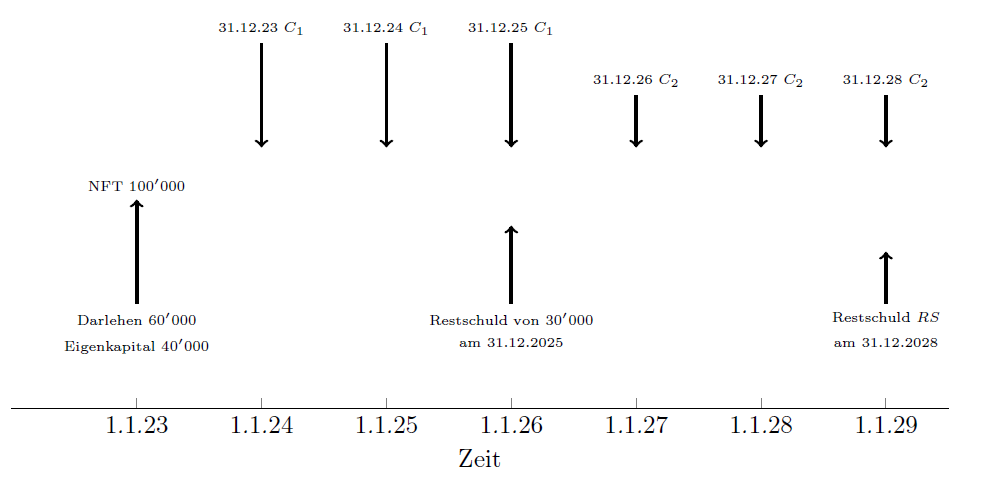
\includegraphics[scale=0.55]{pictures/zeitstrahl_1_b_filled_1}
\end{center}

\underline{(b2) Bestimme die Höhe der Ratenzahlung $ C $}\\


\underline{(b4) Bestimme die restliche Laufzeit mit Hilfe der Restschuld}\\

\underline{(b5) Bestimme die letzte Rate}\\

\newpage
\subsection*{\aufgabe{c}{10}}
Die Alterung der Bevölkerung hat bedeutende ökonomische und soziale Auswirkungen. Deshalb ist es für die Politik von hoher Bedeutung, ein umfassendes Verständnis davon zu haben, wie sich das Bevölkerungswachstum über die nächsten 50 Jahre entwickeln wird.
Modelle des Bevölkerungswachstums sind eine mathematische Beschreibung, wie die Bevölkerung voraussichtlich in Zukunft wachsen wird.
Eines dieser Modelle nimmt an, dass die Grösse $s(t)$ einer Bevölkerung zum Zeitpunkt $t \geq 0$ durch die folgende mathematische Formel beschreiben lässt:
\begin{align*}
	s(t)
	=
	\left(s_0^{1- \gamma} + \mu (1 - \gamma)  t \right)^{\frac{1}{1- \gamma}},
\end{align*}
wobei $s_0 = s(0)$ die Grösse der Bevölkerung zum Zeitpunkt $0$ ist und $\mu, \gamma > 0, \ \gamma \neq 1$ gegebene Parameter sind.
\begin{enumerate}
	\item[(c1)] Berechnen Sie die Wachstumsrate $ \rho_s(t) $ von $ s $.
	\item[(c2)] Benutzen Sie unter der Annahme, dass $s(0) = 10'000 $ Individuen, $\mu = 10$, und $\gamma = 0.5$, die Ableitung von $s$, um die relative Änderung der Bevölkerung zwischen dem Zeitpunkt $t_0 = 5 $ und dem Zeitpunkt $t_0 + \Delta t = 6$ zu approximieren.
\end{enumerate}
\ \\
\textbf{Lösung:}
\begin{mdframed}
\underline{\textbf{Vorgehensweise:}}
\begin{enumerate}
\item[(c1)] 
\begin{enumerate}
	\item[1.] Bestimme die erste Ableitung von $s$.
	\item[2.] Bestimme die Wachstumsrate.
\end{enumerate}
\item[(c2)] Gebe die relative Änderung an und verwende die erste Teilaufgabe.
\end{enumerate}
\end{mdframed}

\underline{(c1) 1. Bestimme die erste Ableitung von $s$.}\\
Die erste Ableitung von $s$ ist mit der Kettenregel gegeben durch
\begin{align*}
	s^\prime(t) = 
	\frac{1}{1- \gamma} 
	\left(s_0^{1-\gamma} + \mu(1-\gamma) t\right)^{\frac{1}{1- \gamma} -1 } 
	(\mu(1-\gamma)).
\end{align*}
\ \\
\underline{(c1) 2. Bestimme die Wachstumsrate.}\\
Die Wachstumsrate von $s$ ist gegen durch
\begin{align*}
	\rho_s(t) = \frac{s^\prime(t)}{s(t)}. 
\end{align*}
Damit folgt:
\allowdisplaybreaks
\begin{align*}
	\rho_s(t) = \frac{s^\prime(t)}{s(t)}
	&=
	\frac{
	\frac{1}{1- \gamma} 
	\left(s_0^{1-\gamma} + \mu(1-\gamma) t\right)^{\frac{1}{1- \gamma} -1 } 
	(\mu(1-\gamma))
	}{
	\left(s_0^{1- \gamma} + \mu (1 - \gamma)  t \right)^{\frac{1}{1- \gamma}}
	}\\
	&=
	\frac{
		\frac{1}{1- \gamma} 
		\left(s_0^{1-\gamma} + \mu(1-\gamma) t\right)^{\frac{1}{1- \gamma} -1 } 
		(\mu(1-\gamma))
	}{
		\left(s_0^{1- \gamma} + \mu (1 - \gamma)  t \right)^{\frac{1}{1- \gamma}}
	}\\
	&=
	\frac{
		\frac{1}{1- \gamma} 
		\left(s_0^{1-\gamma} + \mu(1-\gamma) t\right)^{\frac{1}{1- \gamma}} 
		\left(s_0^{1-\gamma} + \mu(1-\gamma) t\right)^{ -1 }
		(\mu(1-\gamma))
	}{
		\left(s_0^{1- \gamma} + \mu (1 - \gamma)  t \right)^{\frac{1}{1- \gamma}}
	}\\
	&=
		\frac{1}{1- \gamma} 
		\left(s_0^{1-\gamma} + \mu(1-\gamma) t\right)^{ -1 }
		(\mu(1-\gamma))\\
	&=
		\left(s_0^{1-\gamma} + \mu(1-\gamma) t\right)^{ -1 }
		\mu
\end{align*}
\ \\
\underline{(c2) Gebe die relative Änderung an und verwende die erste Teilaufgabe}\\
Die relative Änderung der Bevölkerung zwischen den Zeitpunkten $t_0=5 $ und $t_0 + \Delta t = 6$ ist durch 
\begin{align*}
	\frac{\Delta s}{s(t_0)}
	=
	\frac{s(t_0 + \Delta t) - s(t_0)}{s(t_0)}
\end{align*}
gegeben. Hierbei gilt $t_0 + \Delta t = 6 \ \Leftrightarrow \ \Delta t = 1$.
Die absolute Änderung $\Delta s$ können wir mithilfe der Ableitung von $s$ approximieren:
\begin{align*}
	s^\prime(t_0) \approx \frac{s(t_0 + \Delta t) - s(t_0)}{\Delta t}
	= \frac{\Delta s}{\Delta t}
	\ 
	\Leftrightarrow 
	\
	\Delta s \approx s^\prime(t_0) \Delta t. 
\end{align*}
Damit erhalten wir mit der Wachstumsrate aus (c1):
\begin{align*}
	\frac{\Delta s}{s(t_0)}
	&\approx 
	\frac{s^\prime(t_0 ) \Delta t}{s(t_0)}
	=
	\frac{s^\prime(t_0 ) }{s(t_0)}\underbrace{\Delta t}_{=1}
	=
	\rho_s(t_0) = 
	\frac{\mu}{s_0^{1- \gamma} + \mu (1- \gamma) t_0}\\
	&=
	\frac{10}{10000^{1 - 0.5} + 10 ( 1- 0.5)5 }
	=
	\frac{10}{\sqrt{10000} + 25 }\\
	&=
	\frac{10}{125}
	= 
	\frac{2}{25}
	= 
	\frac{8}{100} = 8 \%.
\end{align*}
\ \\
Alternativ können wir die Aufgabe auch ausschließlich mit der Ableitung von $s$ (ohne die Wachstumsrate zu verwenden) lösen. Mit obiger Approximation gilt
\begin{align*}
	\Delta s &\approx s^\prime(t_0) \underbrace{\Delta t}_{=1}
	=
	\mu \left(
		s_0^{1-\gamma} + \mu (1- \gamma) t_0
	\right)^{\frac{1}{1- \gamma} - 1}\\
	&=
	10 \left(
	10000^{0.5} + 10 (1- 0.5) 5
	\right)^{\frac{1}{1- 0.5} - 1}\\
	&=
	10 \left(
	100 + 25
	\right)^{2 - 1}
	=
	10 \cdot 125 
	=
	1250.
\end{align*}
Für die relative Änderung benötigen wir noch $s(t_0)$:
\begin{align*}
	s(t_0)
	= 
	s(5)
	= 
	(10000^{0.5} + 10 \cdot 0.5 \cdot 5)^{\frac{1}{0.5}} 
	= 
	(100 + 25)^2 
	=
	15625.
\end{align*}
Damit erhalten wir:
\begin{align*}
	\frac{\Delta s}{s(t_0)}
	\approx
	\frac{1250}{(100 + 25)^2 }
	=
	\frac{10 \cdot 125}{125^2}
	= \frac{10}{125} = \frac{8}{100} = 8 \%.
\end{align*}

